\subsection{Verbindungsmöglichkeit }\label{Verbindung}
\SecAuth{\nameCZ}
In Bezug auf die Teststation sollen alle Daten der Sensorik extern über ein drahtloses Verfahren auf einem Laptop/PC empfangen werden, da eine serielle Verbindung durch das Gyroskop in der Teststation viele Komplikationen mit sich bringt. Die Möglichkeiten für solch einen drahtlosen Empfang sind TCP, UDP oder Bluetooth. \\
\vspace{3mm}
Da der CM3+ im Cubesat kein WLAN/Bluetooth-Modul aufweist, muss ein externes Modul über die USB2.0 Schnittstelle am Raspberry PI angeschlossen werden. Ein sogenannter „Dongle“ (USB/Wifi-Bluetooth Modul) wird hierbei verwendet. Da keine normale USB-Buchse am CM3+ angebracht ist (siehe Abb. 88), muss der Dongle mit dem CM3+ durch eine andere Möglichkeit verbunden werden. Das Erstellen einer Buchse für die Verbindung des Dongles wäre hier von Vorteil. \\
\vspace{3mm}
\begin{figure}[H]
	\centering
	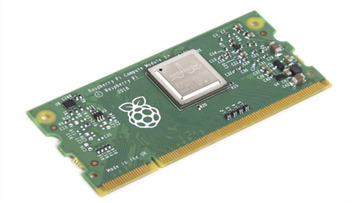
\includegraphics[scale=0.8]{image/cm3+.png}
	\caption{Bild des CM3+ von Raspberry PI}
\end{figure}
\vspace{3mm}
\subsubsection{UDP}\label{udp}
Da für die Simulation des Cubesats ein Raspberry PI 4 benutzt wurde, konnte zuerst das WIFI-Modul auf dem Einplatinencomputer verwendet werden. Für die Kommunikationsmethode wurde dafür das UDP-Protokoll genutzt, welches eine schnelle Datenübertragung sicherstellt. UDP\autocite{UDP} dient als minimales Netzwerkprotokoll, das sich für das Versenden von Datenpaketen über das Internet eignet. UDP verwendet keine Handshakes, um eine Verbindung zwischen zwei Endgeräten herzustellen. Dies bedeutet, dass Daten ohne vorherige Kommunikation gesendet werden. Das Protokoll führt zu einer schnelleren Übertragung als TCP, ist jedoch beim Datentransfer unzuverlässiger.

\subsubsection{TCP}
TCP\autocite{TCP} (transmission control protocol) bietet auch eine gute Übertragungsmöglichkeit, da es mit der Hilfe von dem „Handshake-Vereinbarung“ (siehe Abb. 89) eine fehlerfreie Übertragung des Pakets garantiert. Durch die längere Sendezeit des TCP-Protokolls eignet sich das Protokoll für eine zeitkritische Aufnahme von Daten, wie bei der Teststation vorhanden, nicht.\\
\vspace{3mm}
\begin{figure}[H]
	\centering
	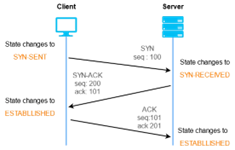
\includegraphics[scale=1.1]{image/sendeverfahren.png}
	\caption{Sendeverfahren des TCP-Protokolls\autocite{TCP-Handshake}}
\end{figure}
\vspace{3mm}
Bei dem „Dreifach Handshake Verfahren“, werden SYN- und ACK-Pakete zwischen zwei Endgeräten ausgetauscht. Der Austausch beginnt mit einem SYN-Paket des Clients, gefolgt von einem SYN-ACK-Paket des Servers. Anschließend wird noch ein ACK-Paket vom Client zum Server geschickt. Durch diese Reihenfolge wird sichergestellt, dass Datenpakete in der richtigen Reihenfolge und ohne Fehler übertragen werden. Auch ermöglicht das Protokoll eine Flusskontrolle, um möglichen Datenstau zu vermeiden.

\subsubsection{Serielle Verbindungsmöglichkeit}
Beginn wurde eine Verbindung über die Schnittstelle UART probiert. Hierbei wird der Raspberry PI über die RX und TX-Pins mit einem Serial/USB Adapter mit einem PC verbunden.\\
\vspace{3mm} 
Damit solch eine Verbindung funktioniert müssen die Jumper-Kabel so angeschlossen werden, dass der RX-Pin des Senders mit dem TX-Pin des Empfängers und der TX-Pin des Senders mit dem RX-Pin des Empfängers verbunden ist.\\
\vspace{3mm}
Anschließend lässt sich über die PySerial Bibliothek eine serielle Verbindung erstellen. Für die Datenaufnahme am PC können verschiedene Programme wie TerraTerm oder RealTerm verwendet werden. Auch kann ein eigenes Programm geschrieben werden, welches den Prozess kontrollierbarer macht. \\
\vspace{3mm}
Für die Testung der Verbindung wurde ein kleines Programm auf dem Raspberry PI entwickelt, welches Daten über die serielle Schnittstelle sendet und vom Computer über TerraTerm empfangen wird. Für solch ein Skript muss zuerst der serielle Port des Raspberry Pis geöffnet werden. Dies kann über das Interface Menu in der Raspberry PI Config unter „sudo raspi-config“ eingestellt werden. Der Name des Ports und alle anderen offenen Ports lassen sich unter „/dev  \$ ls“ anzeigen. 
\vspace{3mm}
Nun kann mit der Python Library „PySerial“ die Verbindung aufgebaut werden:
\begin{itemize}
	\item Zuerst muss ein Serial-Objekt erstellt werden:
	ser = serial.Serial('/dev/ttyS0', 9600)
	\begin{verbatim}
		#Serial Port tty0 wird geöffnet mit einer Baud Rate von 9600
	\end{verbatim}
	
\end{itemize}
\begin{itemize}
	\item Für das Testen der seriellen Verbindung wurden nur Strings zum Laptop geschickt. Dies funktioniert über:
	\begin{verbatim}
		while True:
		ser.write(b‘Test\n') #Sendet den String Test 
		time.sleep(1) # Wartet eine Sekunde
	\end{verbatim}
	\item Damit das Programm nicht endlos läuft, wurde noch ein Keyboard-Interrupt eingebaut. Dies stoppt das Programm, sobald die Tastenkombination strg+c gedrückt wird.
	\begin{verbatim}
		except KeyboardInterrupt:
		ser.close()  
		# Schließt die serielle Verbindung, 
		sobald das Programm unterbrochen wird.
	\end{verbatim}
\end{itemize}
Sobald das Skript gestartet wird, fängt der Raspberry PI an, Daten an den Laptop zu senden, wo sie anschließend von TerraTerm aufgenommen werden.

\newpage
\subsection{Übertragungsmethode } \label{über}
Nach weiterer Überlegung und Analyse wurde UDP gegenüber TCP oder einer seriellen Verbindung bevorzugt. Dies liegt daran, dass UDP weniger Overhead hat und daher schneller ist. Es bietet auch eine große Flexibilität, da es keine Verbindung herstellen oder aufrechterhalten muss, was zu einer verbesserten Leistung führen kann.\\
\vspace{3mm}
Eine Übertragung von Paketen in UDP, unter bestimmten Umständen kann auch sicherheitsrelevant sein. Insbesondere wenn es um die Integrität, Verfügbarkeit und Vertraulichkeit der Daten geht. Es ist jedoch möglich, diese Sicherheitsrisiken zu mindern, indem man zusätzliche Sicherheitsmaßnahmen und Protokolle implementiert, die für den jeweiligen Anwendungsfall geeignet sind. \\
\vspace{3mm}
Um eine Verbindung zwischen dem Raspberry PI und dem Computer herzustellen, müssen sich beide Endgeräte im gleichen Netz befinden. Auch sollten beide Systeme die IP-Adresse des anderen im Voraus wissen. 

\subsubsection{Senderoutine }\label{sende}
Das Python Skript, welches sich auf dem Raspberry PI befindet, ist für das Senden der Sensordaten zuständig, welche über I²C vom EDU-HAT abgelesen werden. Für die I²C Kommunikation mit der Sensorik wird eine Bibliothek der TU-Wien namens STS1\_Sensors.py verwendet. Wie die Auslesung über I2C im Programm funktioniert, wird im Kapitel \ref{i2C} noch genauer behandelt.\\
\vspace{3mm}
Um die UDP-Verbindung herzustellen, wird die „sockets“ Bibliothek von Python benötigt. Sie erlaubt es, Daten über das Internet-Protokoll zu senden und zu empfangen. Sockets sind Endpunkte einer bidirektionalen Kommunikationslinie zwischen zwei Programmen, die auf dem Netzwerk laufen.\\
\vspace{3mm}
Die „time“ Bibliothek ist auch ein wichtiger Bestandteil dieses Programms. Sie ermöglicht das Anhalten des Programms für eine bestimmte Anzahl von Sekunden. \\
\vspace{3mm}
Eine weitere Bibliothek, die für dieses Programm nützlich ist, ist die „json“ Library. Speziell die Funktion „json.dumps()“ ,welche es ermöglicht  um ein Python-Objekt (in unserem Fall ein String) in eine JSON-Zeichenkette umzuwandeln. JSON ist leicht lesbar und einfach zu verstehen, was uns beim Schreiben der CSV-Datei deutlich hilft. 
\newpage
\subsubsection{Programm SensorOut.py}\label{out}
Dies ist das Programm für die Senderoutine wie in Kapitel \ref{sende} genannt. In diesem Kapitel wird nur das UDP-Sendeverfahren genau besprochen. In Kapitel \ref{udp} werden genauere Informationen über den Vorgang der Datenauslesung dargestellt. \\
\vspace{3mm}
Um die UDP-Verbindung zu erstellen, muss der Raspberry PI wissen, an wen er die Pakete schicken muss. Die Zieladresse und Portnummer sind als Variable angegeben, damit ein Benutzer sie leicht verändern kann.
\begin{itemize}
	\item udp\_ip = '172.20.10.3' \#Zieladresse: Kann verändert werden 
	\item udp\_port = 50687 \#Portnummer: Kann verändert werden
\end{itemize}
Es ist wichtig zu wissen, dass die Zieladresse immer die Adresse sein muss, bei welcher die Daten empfangen werden sollen. Die Portnummer muss bei Sender und Empfänger gleich gewählt werden.\\
\vspace{3mm} Ansonsten werden keine Daten am Empfänger ankommen.
Da ohne ein Interrupt die Arbeitsschleife des Systems endlos laufen würde, muss eine BOOL Variable erstellt werden, welche abfragt, ob ein Interrupt eingetroffen ist. 
\vspace{3mm}
\begin{figure}[H]
	\centering
	\begin{minted}{python}
		# Flag Controlling für den Loop
		running = True
		try:
		while running:
		# Rest des Codes 
		
	\end{minted}
\end{figure}
\vspace{3mm}
Man kann sehen, dass während das BOOL „running“ den Zustand „True“ besitzt, die Arbeitsschleife ausgeführt wird.  Sobald jedoch ein KeyboardInterrupt auftritt, wird die Schleife gestoppt und ist nur durch einen Neustart des Programms wieder ausführbar.
\vspace{3mm}
\begin{figure}[H]
	\centering
	\begin{minted}{python}
		except KeyboardInterrupt:
		# Programm stoppt sobald strg+c gedrückt wird
		running = False #Running flag auf False
		print("Loop stopped by user.") 
		#Meldung, dass das Programm abgebrochen wurde
	\end{minted}
\end{figure}
Running ist nun auf FALSE und entspricht nicht mehr der Bedingung, welche oben genannt wurde.\\
Die UDP-Senderoutine befindet sich in der Hauptschleife des Programms. Zuerst wird über einen Konstruktor ein neues Socket-Objekt erzeugt. Dieses erstellt einen neuen Socket für die Verwendung mit UDP.
\vspace{3mm}
\begin{figure}[H]
	\centering
	\begin{minted}{python}
		# UDP-Socket erstellen und öffnen 
		sock = socket.socket(socket.AF_INET, socket.SOCK_DGRAM) 
	\end{minted}
\end{figure}
“socket.AF\_INET” ist dabei die Adressfamilie, über welche das UDP-Paket verschickt wird. In diesem Beispiel wird das Pakket über IPv4 verschickt. Der Begriff „socket.SOCK\_DGRAM“ gibt an, dass die Versendungsmethode UDP sein soll.\\
\vspace{3mm}
Anschließend können die Sensordaten über den Socket verschickt werden. 
\vspace{3mm}
\begin{figure}[H]
	\centering
	\begin{minted}{python}
		# Daten über UDP-Socket schicken 
		sock.sendto(data_string.encode(), (udp_ip, udp_port))
		
	\end{minted}
\end{figure}
Die Methode “sock.sendto” versendet den Daten String zu der oben ausgemachten Ziel IP-Adresse über den auch ausgemachten Port \\

Zum Schluss schließt sich der Socket und es wird eine beliebige Anzahl von Sekunden gewartet. Die Zeit kann bei einer oben angelegten Variable („t\_sleep“), je nach Schnelligkeit der Messung, umgeändert werden. \\
\vspace{3mm}
\begin{figure}[H]
	\centering
	\begin{minted}{python}
		Die Variable t\_sleep:
		# Konfiguration der Wartezeit 
		t_sleep = 5 #Wartezeit: Kann verändert werden 
		
		Schließung des Sockets und Verwendung der Wartezeit:
		sock.close() #Schließen des Sockets nach dem Senden
		#Warten für t_sleep Sekunden
		time.sleep(t_sleep)
		
	\end{minted}
\end{figure}
\newpage
Dies ist der Ablauf der Senderoutine auf dem Raspberry PI. Das Programm ist eine Endlosschleife, welche sich nur durch das Ausschalten des Raspberry PI‘s oder durch die Verwendung des eingebauten Keyboard Interraps (strg+c) unterbrechen lässt.\\
\vspace{3mm}
Das gleiche Programm wurde für das Senden für die Sensordaten der Teststation umgeschrieben. Die Senderoutine ist gleich aufgebaut wie oben erklärt mit dem Unterschied, dass weniger Daten gesendet werden.

\subsection{Empfangsroutine }\label{empfang}
Das zweite Modul, was für eine erfolgreiche UDP-Verbindung verwendet werden muss, ist ein Skript namens „UDPsniff.py“ auf dem Computer, welches die gesendeten Daten empfängt und in eine CSV-Datei einschreibt.\\
\vspace{3mm}
Der Empfang funktioniert in etwa gleich wie das Senden von UDP-Paket. Wie im genannten Skript (siehe: Kap \ref{out}) wird für das Empfangen die „Sockets“ Bibliothek von Python verwendet. \\
\vspace{3mm}
Wie schon zuvor wird die IP-Adresse und der UDP-Port außerhalb der Arbeitsschleife angegeben. Auch wird der Socket geöffnet und die Adresse sowie Port dem Socket zugewiesen:
\vspace{3mm}
\begin{figure}[H]
	\centering
	\begin{minted}{python}
		# UDP setup
		udp_ip = "0.0.0.0" 
		#Jede IP-Adresse auf dem Port zuhören
		udp_port = 50687 
		#Port muss gleich wie auf dem Raspi sein
		sock = socket.socket(socket.AF_INET, socket.SOCK_DGRAM) 
		#Code zeile   wurde in Kap 2.4.1 erklärt
		sock.bind((udp_ip, udp_port))
		#IP und Port dem Socket zuweisen
		
		
	\end{minted}
\end{figure}
In diesem Beispiel wird erlaubt, dass für jede IP-Adresse auf dem Port 50687 gehört wird. Falls mehrere IP-Adressen schon über den gegebenen Port kommunizieren, wäre es vorteilhaft die IP-Adresse auf die IP-Adresse des Senders umzuändern. Wie in Kap: \ref{out} schon genannt ist es wichtig, dass der UDP-Port des Senders und Empfängers identisch ist, da sonst keine Daten empfangen werden können.\\
\vspace{3mm}
Die Daten des Programms werden in der Arbeitsschleife des Programms empfangen. Die Funktion dafür lautet:
\vspace{3mm}
\begin{figure}[H]
	\centering
	\begin{minted}{python}
		data, addr = sock.recvfrom(1024)  
		#Warten auf Date -> Buffer size 1024
		print(f"Data received from {addr}") 
		#Anzeigen von welcher IP-Adresse das Paket
		#kommt
	\end{minted}
\end{figure}
Die erste Zeile des Code Abschnitts wartet auf ein einkommendes UDP-Paket. Die maximale Größe dieser Daten ist durch die Buffer-Size auf 1024 Bits, begrenzt. Sobald ein Paket auf den angegebenen Port und von der angegebenen IP-Adresse eintrifft, werden die Daten sowie die Sende-Adresse abgespeichert. Für die Prüfung der Korrektheit wird angegeben, von welcher IP-Adresse des Pakets versendet wurde. \\
\vspace{3mm}
Anschließend werden die Daten separiert und in eine CSV-Datei eingespeichert. Dies wird in einem anderen Kapitel (Kapitel \ref{csv}) noch genauer erklärt.\\
\vspace{3mm}
Um das Programm zu beenden, wurde ein Keyboard Interrupt eingebaut. Da bei UDP möglicherweise Fehler beim Senden entstehen können, wurden auch verschiedene „Exceptions“ eingebaut. Exceptions reagieren auf Ausnahmen und Fehler, die während der Ausführung des Codes aufkommen können. 
\vspace{3mm}
\begin{figure}[H]
	\centering
	\begin{minted}{python}
		except KeyboardInterrupt:
		print("\nScript terminated by user.")
		except Exception as e:
		print(f"An error occurred: {e}")
		finally:
		sock.close()
		print("Socket closed.")
		
	\end{minted}
\end{figure}
Die Code Zeile “except Exeption as e:“ reagiert auf die Fehler, die im Code auftreten können. Anschließend wird der Fehler auf die Variable gespeichert und im Terminal dargestellt. \\
\vspace{3mm}
Mit der Anwendung von „finally:“ wird der Socket automatisch nach dem Vorkommen eines Fehlers geschlossen, um einen Netzwerkstau am Port zu vermeiden. \\
\vspace{3mm}
Nachdem die Daten angekommen sind, werden sie noch im Terminal als Kontrolle dargestellt:\\
\begin{verbatim}
	Data received from ('192.168.345.241', 52047)
	#Angabe von wo die Daten gesendet wurden
	Decoded Data: {'Temperature (TMP112)': 23.9375,
	'Temperature (BME688)': 24.32558551326565,
    'Humidity': 41.17989757653827, 
    'Pressure': 96206.06435710512, 
    'Gas Resistance': 71688.60263231589,
    'Acceleration X': -253, 
    'Acceleration Y': 4, 
    'Acceleration Z': -2, 
    'Gyroscope X': -0.9902152641878669, 
    'Gyroscope Y': 0.015655577299412915, 
    'Gyroscope Z': -0.007827788649706457, 
    'UVA': 13, 'UVA Index': 0} 
    #Darstellung der dekodierten Daten
\end{verbatim}
\vspace{3mm}

\subsubsection{Schreiben der Daten in eine CSV-Datei}\label{csv}
Nachdem die Daten am Empfänger angekommen sind, werden sie in eine CSV-Datei geschrieben. Eine CSV-Datei ist eine Textdatei, die Daten in Form einer Tabelle speichert. Jede Zeile in der CSV-Datei entspricht einer Zeile in einer Tabelle. Die einzelnen Werte (Zellen) in dieser Zeile sind durch Kommas getrennt (Abb. 90-91).  CSV eignet sich gut für den Datenaustausch zwischen Programmen. Dies ist besonders vorteilhaft, da hier separate Programme für das Einlesen und  das Visualisieren von Daten verwendet werden.
\vspace{3mm}
\begin{figure}[H]
	\centering
	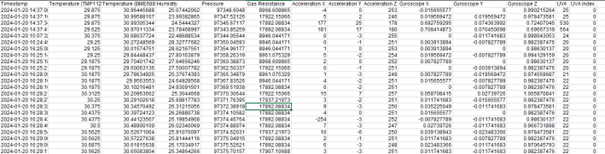
\includegraphics{image/tabellen.png}
	\caption{Tabellenform}
\end{figure}
\vspace{3mm}
\begin{figure}[H]
	\centering
	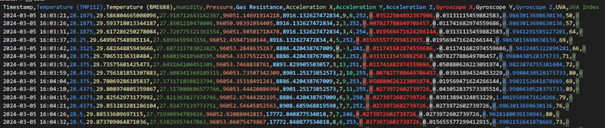
\includegraphics{image/darstellung.png}
	\caption{Darstellungsweise der CSV-Datei}
\end{figure}

\subsubsection{CSV-Datei Programm}
Das Programm, welches für das Schreiben der CSV-Datei zuständig ist, ist dasselbe wie jenes, das für das Empfangen des UDP-Pakets verantwortlich ist („UDPsniff.py“). Somit werden alle empfangenen Daten gleich in die CSV-Datei eingeschrieben. Dafür muss zuerst eine Datei erstellt und ihr Pfad angegeben werden:
\vspace{3mm}
\begin{figure}[H]
	\centering
	\begin{minted}{python}
		# Pfad der CSV-Datei
		csv_file_path='C:\\Users\\Constantin\\Documents
		\\5BHEL\\Diplomarbeit\\DashboardSTS1
		\\udp_data.csv'
		
	\end{minted}
\end{figure}
Wo genau die CSV-Datei liegt, ist egal, solange der genaue Pfad angegeben wird. \\
Anschließend werden die Kopfzeilen („Headers“) definiert. Diese müssen identisch zu den Titeln der empfangenen Daten sein, da das Programm, je nach Titel, die Werte zu dem angegebenen Header sortiert.
\vspace{3mm}
\begin{figure}[H]
	\centering
	\begin{minted}{python}
	# Definition der Headers
	headers = 
	["Timestamp", "Temperature (TMP112)",
	"Temperature (BME688)", 
	"Humidity", 
	"Pressure",
	"Gas Resistance", 
	"Acceleration X", 
	"Acceleration Y", 
	"Acceleration Z",
	"Gyroscope X", 
	"Gyroscope Y", 
	"Gyroscope Z", 
	"UVA", "UVA Index"]	
	\end{minted}
\end{figure}
Nicht in dem UDP-Paket vorhanden ist der Header: „Timestamp“. Dieser wird benötigt, um die Zeit zu erfassen, zu der die Daten empfangen wurden. Der Header wird manuell hinzugefügt, um die Sensordaten bei der Visualisierung zeitlich einzuordnen und um zu analysieren, wie sich die Sensorwerte im Laufe der Zeit verändern. \\
\vspace{3mm}
Anschließend wird in einem „try“-Block, welcher für das Abfragen von Ausnahmezuständen zuständig ist, die CSV-Datei geöffnet.
\vspace{3mm}
\begin{figure}[H]
	\centering
	\begin{minted}{python}
		#Öffnen der CSV-Datei im Modus a
		with open(csv_file_path, mode='a', newline='') as file:
		# Überprüft, ob die Datei leer ist
		file_empty = file.tell() == 0
		#Erstellen eines CSV wirter Objekts
		
	\end{minted}
\end{figure}
Die erste Zeile dieses Codeabschnitts öffnet die angegebene Datei, welche sich am Pfad ‚csv\_file¬\_path‘ befindet. Der Modus bestimmt, wie die Daten eingelesen werden sollen. Der Modus ‚a‘ gibt an, dass neu einkommende Daten an das Ende der Datei angehängt werden, ohne schon eingeschriebene Inhalte zu überschreiben. Der Modus ‚a‘ kann aber auch verwendet werden, um eine noch nicht existierende Datei zu erstellen. \\
\vspace{3mm}
Der Parameter „ newline=‘ ‘ “ wird verwendet, um sicherzustellen, dass die Zeilenumbrüche korrekt gehandhabt werden. Dies ist besonders wichtig, falls die Datei zwischen mehreren Betriebssystemen geteilt wird. Das oben geöffnete Dateiobjekt ‚open ()‘ wird der Variable ‚file‘ zugewiesen, die innerhalb des „with“ Blocks verwendet wird.\\
\vspace{3mm}
‚file.tell()‘ gibt die aktuelle Position in der CSV-Datei zurück. Hier wird durch, „file.tell() == 0“ abgefragt, ob die CSV Datei leer ist.\\
\vspace{3mm}
Anschließend wird ein. ‚csv.writer()‘ Objekt erstellt, das für das Schreiben von Daten in das ‚file‘-Objekt verwendet wird.
\vspace{3mm}
\begin{figure}[H]
	\centering
	\begin{minted}{python}
		#Erstellen eines CSV writer Objekts
		writer = csv.writer(file)
		
	\end{minted}
\end{figure}
Da ein leeres File keine Kopfzeilen besitzt wird, falls die Datei leer ist, alles Headers eingeschrieben.
\vspace{3mm} 
\begin{figure}[H]
	\centering
	\begin{minted}{python}
		if file_empty: 
		#Falls die CSV Datei noch leer ist
		writer.writerow(headers) 
		#Headers als in erste Reihe einfügen
	\end{minted}
\end{figure}
Dafür wird zuerst abgefragt, ob die oben definierte BOOL ‚True‘ ist. Falls dies der Fall ist, werden alle Header, welche zuvor beschrieben wurden, in die erste Reihe der CSV-Datei geschrieben.\\
\newpage
In der Arbeitsschleife werden die empfangenen Daten dekodiert und in die CSV-Datei geschrieben: 
\vspace{3mm} 
\begin{figure}[H]
	\centering
	\begin{minted}{python}
		try:
		#Daten in einen String konveriten
		decoded_data = data.decode()
		#Daten für die Verarbeitung 
		in ein JSON-Objekt umwandeln
		sensor_data = json.loads(decoded_data)
		#Ausgabe der dekodierten Daten
		print(f"Decoded Data: {sensor_data}")
		#Erzeugung eines Zeitstempels 
		current_time = 
		datetime.now().strftime("%Y-%m-%d %H:%M:%S")
		
		# Für jeden Zeitstempel werden die Sensordaten eingefügt
		writer.writerow([current_time] +
		[sensor_data.get(key, '') for key
		in headers[1:]])
		#Buffer der Datei löschen, 
		damit Daten sofort geschrieben werden
		file.flush()
		
	\end{minted}
\end{figure}
Da der Code potenziell eine Ausnahme (Exception) werfen könnte, beginnt die Arbeitsschleife mit einem ‚try:‘ Block. Falls während der Ausführung des Blocks eine Ausnahme auftritt, kann das Programm gleich zu der gegebenen Exception springen. \\
\vspace{3mm}
Um die Daten wieder in ein String Format zu konvertieren, werden die empfangenen Daten mit der Methode ‚.decode()‘ dekodiert und auf die Variable ‚decoded\_data‘ abgespeichert. \\
\vspace{3mm}
Anschließend werden die dekodierten Daten für das Einschreiben in die Datei in ein „JSON-Objekt“ umgewandelt und als die Variable ‚sensor\_data‘ gespeichert. Obwohl dies schon im Programm der Senderoutine (siehe: Kap. \ref{out}) gemacht wurde, wurde der String für das Senden über UDP in Byte-Daten umgewandelt. Es ist trotzdem wichtig, dass der String ‚decoded\_data‘ im JSON-Format geschrieben ist, da die Operation ‚json.loads()‘ voraussetzt, dass dieser eine gültige JSON-Zeichenkette ist.\\
\vspace{3mm} 
Auf die Variable „current\_time“ wird durch die Funktion ‚datetime.now()‘ die aktuelle Zeit in einen String abgespeichert. Auch wird das Format der Zeit angegeben (Jahr-Monat-Tag Stunde: Minute:Sekunde).\\
\vspace{3mm}
In dem nächsten Abschnitt wird mit der Funktion, „writer.writerow()“ eine Zeile der CSV-Datei geschrieben.  Zuerst wird die aktuelle Zeit in die Zeile geschrieben. Anschließend werden die Werte von ‚sensor\_data‘ geschrieben, welche den Titeln der Kopfzeilen entsprechen. \\
\vspace{3mm}
Falls ein bestimmter Wert nicht mit dem Header übereinstimmt, wird ein leerer String eingefügt. Der Codeabschnitt, ‚headers [1:]‘ deutet darauf hin, dass das erste Element in ‚Headers‘ übersprungen wird, da diese Spalte für die Zeit reserviert ist.\\
\vspace{3mm}
Um einen möglichen Datenstau bei schnellerem Senden und Empfangen zu vermeiden, wird durch die Funktion ‚file.flush()‘,das System, gezwungen, alle gepufferten Daten sofort in die CSV-Datei zu schreiben. \\
\vspace{3mm}
Da das Programm durch die Implementierung von JSON-Dekodierung anfällig auf Ausnahmen (Exzeption) sein kann, werden die möglichen Fehler am Schluss des Codes noch abgefangen und aufgeschrieben. Dies wurde auch für generelle Ausnahmen, außerhalb der JASON-Dekodierung, gemacht. 
\vspace{3mm} 
\begin{figure}[H]
	\centering
	\begin{minted}{python}
		except json.JSONDecodeError as e: 
		#Apprüfung von Fehlern der JSON-Dekodierung
		print(f"JSON Decode Error: {e}") 
		#Ausgabe des Fehlers 
		except Exception as e: 
		#Apprüfung für allgemeine Fehler
		print(f"Unexpected error: {e}") 
		#Ausgabe der allgemeinen Fehler
		
	\end{minted}
\end{figure}
Durch dieses Programm können nun alle empfangenen Daten in eine CSV-Datei in bestimmter Reihenfolge abgespeichert werden und später für die Visualisierung und Analyse der Daten verwendet werden.
\newpage
\subsubsection{Sensorik mittels I²C-Interface lesen}\label{i2C}
Alle Sensorik, welche sich auf dem EDU befindet, wird mit I2C angesteuert und gelesen. Dies ermöglicht eine effiziente Kommunikation und Datenübertragung zwischen den Sensoren auf dem HAT und dem Raspberry PI. Nach der Realisation verschiedener Python Skripten, die zur Auslesung von den Werten der Sensorik dienten, wurde eine Bibliothek der TU-Wien, Namens „STS1\_Sensors.py“ verwendet, was diesen Prozess vereinfachte.\\
\vspace{3mm}
Eine allgemeine Information ist unter „\url{ti.com/lit/an/slva704/slva704.pdf?ts=1712280198725&ref_url=https%253A%252F%252Fwww.google.com%252F}“ zu finden.\\
\begin{figure}[H]
	\centering
	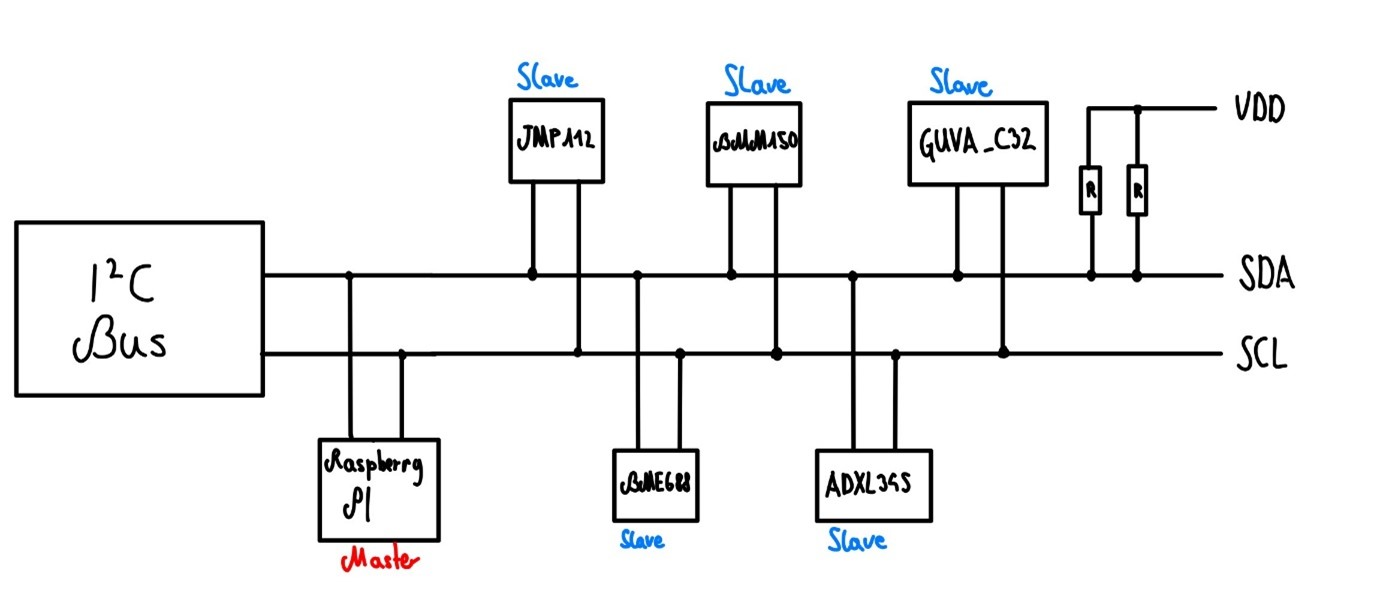
\includegraphics[scale=1.1]{image/constibild.jpg}
	\caption{Aufbau des I2C-Systems auf dem Raspberry PI }
\end{figure}


\subsection{Bibliothek „STS1\_Sensors.py “}\label{bib}
Die Bibliothek „STS1\_Sensors.py“ dient zur Interaktion zwischen dem Raspberry PI und der Sensorik über den I2C-Bus. Das Python Programm verfügt über mehrere Klassen, um mit den Sensoren zu interagieren und um Daten zu lesen. \\
\vspace{3mm}

\begin{itemize}
	\item Die Klasse „SensorsData“ speichert alle Daten, die von den Sensoren gelesen werden. Darunter sind die Temperatur, Luftfeuchtigkeit, Luftdruck, Gaswiderstand, Beschleunigung, Magnetfeldstärke und UV-Strahlung (siehe Kap.: \ref{edu}). Sie ist die wichtigste Klasse für das einfache Auslesen der Sensoren.
	\item Die Klasse „Sensors“ ist für die Initialisierung und Deaktivierung der Sensoren verantwortlich. Auch für das Einrichten der Sensoren und das Sammeln von Daten wird sie benötigt.
	\item In der Bibliothek besitzt auch jeder Sensor eine eigene spezifische Klasse. Diese kann für unterschiedliche Initialisierungsmethoden eines bestimmten Sensors verwendet werden, um Konfigurationsoptionen einzurichten oder um einen Sensor gezielt zu deaktivieren.
\end{itemize}
Da für die Teststation alle Werte der Sensorik überprüft werden müssen, eignet sich das generelle Auslesen aller Sensordaten mehr als das Auslesen eines einzelnen Sensors. Aus diesem Grund wird die Klasse „SensorData“ verwendet. 
\subsection{Auslesen der Sensorik mittels „STS1\_Sensors.py“}\label{aus}
Das Auslesen der Sensorik mittels der Bibliothek „STS\_Sensors.py“ wird in dem Programm „SensorOut.py“ realisiert. Dazu müssen die Bibliothek der Sensoren sowie   auch die Bibliothek für die I2C-Verbindung („smbus2“) in das Programm eingebunden werden.\\
\vspace{3mm}
Um die Verbindung zu ermöglichen, muss der I2C-Bus zuerst initialisiert und anschließend eine Instanz der Sensorklasse kreiert werden. 
\vspace{3mm} 
\begin{figure}[H]
	\centering
	\begin{minted}{python}
		# I2C Bus initialisieren
		bus = smbus2.SMBus(1)
		
		# Instanz der Sensorklasse erstellen
		sensors = Sensors(bus)
		
	\end{minted}
\end{figure}
Anschließend können mit der Funktion ‚sensors.setup()‘ alle Sensoren eingestellt und vorbereitet werden. 
\vspace{3mm} 
Über die Funktion ‚Sensors.getData()‘ werden alle Sensoren nach ihren Werten abgefragt. Die Klasse ‚getData()‘ beschäftigt sich mit dem Sammeln der Daten von allen Sensoren. Diese werden alle als ‚Output‘ Objekt abgespeichert.\\
\vspace{3mm}
Dieses Objekt kann mit ‚data = sensors.output‘ nun als Variable ‚Data‘ in der Hauptschleife des Programms abgespeichert werden. \\
\vspace{3mm}
Anschließend werden alle Daten in ein Dictionary namens ‚sensor\_data‘ eingefügt und strukturiert dargestellt. Um dies zu ermöglichen, wird jedem Wert eine Beschreibung gegeben. 
\vspace{3mm}
\begin{figure}[H]
	\centering
	\begin{minted}{python}
		#Dictionary für die Sensorwerte erstellen
		sensor_data = { "Temperature (TMP112)": data.tempTMP, 
			"Temperature (BME688)": data.tempBME, 
			"Humidity": data.hum, 
			"Pressure": data.press,
			"Gas Resistance": data.gasRes, 
			"Acceleration X": data.accX, 
			"Acceleration Y": data.accY, 
			"Acceleration Z": data.accZ,
			"Gyroscope X": data.gX, 
			"Gyroscope Y": data.gY, 
			"Gyroscope Z": data.gZ, 
			"UVA": data.uva, 
			"UVA Index": data.uvaI }
		
	\end{minted}
\end{figure}
Anschließend werden die Daten mittels UDP an die Zieladresse (Computer) zur Visualisierung verschickt (siehe: Kap.: \ref{sende}). \\
\vspace{3mm}
Ein etwa gleiches Verfahren wurde auch auf für die Sensorik der Teststation entwickelt, damit die Soll- und Istwerte des Cubesats bzw. der Teststation verglichen werden können. \\
\vspace{3mm}
In keinem der Datenblätter für die Sensoren wurde "Clock Stretching" erwähnt. "Clock Stretching\autocite{I2CMode}" ist eine Funktion des IC2-Protokolls, die es einem Slaven ermöglicht, die Taktleitung auf "Low" zu halten, sodass der schnellere Master warten muss.
